\chapter{Projekt i implementacja aplikacji klienckiej oraz REST API}

\section{Funkcje aplikacji}

%TODO: krótki opis

\subsection{Diagram przypadków użycia}

\begin{figure} [H]
	\centering
	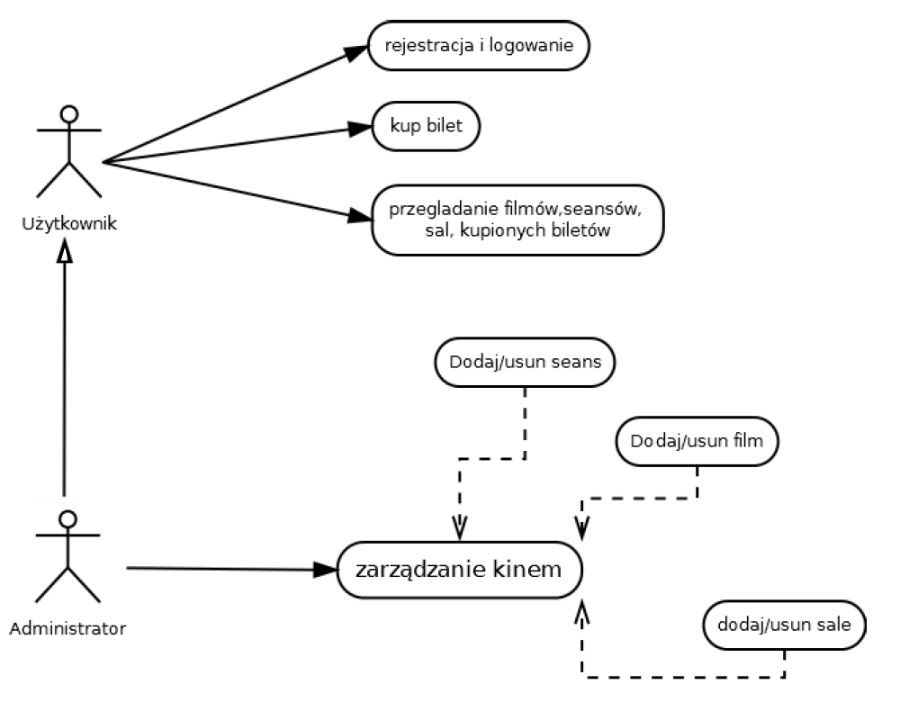
\includegraphics[width=0.6\linewidth]{rozdzial05/diagram.png}
	\caption{Diagram przypadków użycia}
	\label{fig:schem}
\end{figure}

Użytkownik:
\begin{itemize}
	\item tworzenie nowego konta (podanie loginu, hasła itp.);
	\item logowanie;
	\item przeglądanie filmów, seansów, kupionych biletów;
	\item kupowanie biletów.
\end{itemize}

Administrator:
\begin{itemize}
	\item te same funkcjonalności co użytkownik;
	\item dodawanie/usuwanie/edytowanie seansów;
	\item dodawanie/usuwanie/edytowanie filmów;
	\item dodawanie/usuwanie/edytowanie dostępnych sal.
\end{itemize}

\subsection{Scenariusz wybranych przypadków użycia}

W poniższych tabelach umieszczone zostały scenariusze wybranych przypadków użycia.

\begin{table}[H]
	\begin{tabularx}{\textwidth}{ |l|X| }
		\hline 
		Przypadek użycia & Rejestracja  \\ 
		\hline 
		Opis & Funkcja umożliwiająca założenie konta w systemie \\ 
		\hline 
		Warunki początkowe & Brak konta \\ 
		\hline 
		Warunki końcowe & System utworzył konto lub odrzucił żądanie  \\ 
		\hline 
		Przebieg podstawowy & 1. Użytkownik podaje swoje dane (login, hasło itp.) \\ 
		& 2. System sprawdza czy login nie jest zajęty \\
		& 3. Jeśli login jest wolny, skok do pkt 6. \\
		& 4. Wyświetlenie komunikatu o błędach \\
		& 5. Skok do pkt 1. \\
		& 6. Zakończenie rejestracji \\
		\hline 
	\end{tabularx} 
    \caption{Scenariusz rejestracji}
\label{tab:scen1}   
\end{table}

\begin{table}[H]
	\begin{tabularx}{\textwidth}{ |l|X| }
		\hline 
		Przypadek użycia & Logowanie  \\ 
		\hline 
		Opis & Funkcja umożliwiająca użytkownikom uzyskanie dostępu do systemu \\ 
		\hline 
		Warunki początkowe & Posiadanie własnego konta \\ 
		\hline 
		Warunki końcowe & System autoryzował, bądź odrzucił użytkownika  \\ 
		\hline 
		Przebieg podstawowy & 1. Użytkownik podaje swój login i hasło \\ 
		& 2. System wyszukuje użytkownika \\
		& 3. Jeśli użytkownik zostanie zweryfikowany, skok do pkt 6. \\
		& 4. Wyświetlenie komunikatu o błędach \\
		& 5. Skok do pkt 1. \\
		& 6. Zakończenie logowania \\
		\hline 
	\end{tabularx} 
	\caption{Scenariusz logowania}
	\label{tab:scen2}   
\end{table}

\begin{table}[H]
	\begin{tabularx}{\textwidth}{ |l|X| }
		\hline 
		Przypadek użycia & zarządzanie kinem  \\ 
		\hline 
		Opis & Funkcja umożliwiająca pracownikom zarządzanie kinem \\ 
		\hline 
		Warunki początkowe & Funkcja dostępna tylko dla zalogowanych pracowników \\ 
		\hline 
		Warunki końcowe & Dokonanie zmiany w systemie  \\ 
		\hline 
		Przebieg podstawowy & 1. Pracownik uruchamia aplikację zarządzania kinem \\ 
		& 2. Wywołanie odpowiedniego przypadku w zależności od wybranej akcji do wykonania \\
		& 3. Jeżeli wybrano "Dodanie filmu", wywołanie przypadku "Dodanie filmu". Skok do pkt 8. \\
		& 4. Jeżeli wybrano "Dodanie seansu", wywołanie przypadku "Dodanie seansu". Skok do pkt 8. \\
		& 5. Jeżeli wybrano "Usuwanie filmu", wywołanie przypadku "Usuwanie filmu". Skok do pkt 8. \\
		& 6. Jeżeli wybrano "Usuwanie seansu", wywołanie przypadku "Usuwanie seansu". Skok do pkt 8. \\
		& 7. Jeżeli wybrano "Dodawanie sali", wywołanie przypadku "Dodanie sali". Skok do pkt 8. \\
		& 8. Zakończenie procesu \\
		\hline
		Przebieg alternatywny & 1. Pracownik wchodzi na stronę zarządzania kinem. \\
		& 2. Wywołanie odpowiedniego przypadku w zależności od wybranej akcji do wykonania \\
		& 3. Pracownik wylogował się z systemu \\
		& 4. zakończenie procesu. \\
		\hline 
	\end{tabularx} 
	\caption{Scenariusz zarządzania kinem}
	\label{tab:scen3}   
\end{table}

\section{Realizacja wybranych funkcjonalności aplikacji}
%TODO: usunąć wzór
\lssetdef
\lstinputlisting[captionpos=b,caption={Przykładowy listing},label={lst:1},basicstyle={\footnotesize\ttfamily}]{rozdzial05/kod.txt}

%TODO: napisać - PIRU

\section{Realizacja REST API}

%TODO: napisać - PIRU